\chapter{Ciclo de Vida do Sistema}
\section{Definição da Abordagem e Metodologia}
Definiu-se a utilização de uma abordagem de desenvolvimento ágil \cite{beck2001agile} para o contexto inicial do projeto, levando-se em conta que o processo de desenvolvimento seria realizado pelo próprio autor, a disponibilidade do cliente seria mais abrangente e o projeto evoluiria aos poucos, com entregas contínuas de pequenos incrementos de software.

A metodologia utilizada baseou-se no Kanban \cite{radigan_2015}, com algumas práticas do \textit{Extreme Programming}, visto que ambos atendiam de maneira adequada ao fluxo de trabalho contínuo, previsto pela abordagem escolhida.

Para auxiliar nas \textit{releases} do projeto, utilizou-se o conceito de \textit{sprints}, provinda do \textit{Scrum} \cite{scrum_guide}. As \textit{sprints} são pequenos intervalos de tempo, de um mês ou menos, durante o qual uma versão incremental potencialmente utilizável do produto é criada. Uma nova Sprint se inicia imediatamente após a conclusão da Sprint anterior.

Ressalta-se que os próximos tópicos do ciclo de vida não foram completamente realizados em sequência, visto que esses acabavam se intercalando em determinados momentos, como previsto em uma abordagem ágil.

\section{Contexto e Necessidades}
Por questões de disponibilizade e quantidade de equipamentos de medição adquiridos, definiu-se o campus UnB Gama como ambiente de teste para a primeira parte do projeto.

Dois professores doutores, Alex Reis e Loana Nunes Valesco, do campus UnB Gama, foram designados pela Prefeitura de Campus a darem suporte às necessidades energéticas que o sistema deveria atender.

Tendo como problema a falta de monitoramento energético adequado na Universidade de Brasília, foi realizado um estudo mais aprofundado sobre o contexto para identificar as necessidades do cliente. Tal estudo abordava o entendimento de fatores energéticos cruciais, como por exemplo, energia trifásica, horários de ponta e fora de ponta, tensão, corrente, resistência e afins.

A energia elétrica trifásica é um dos métodos mais comuns para se gerar, transmitir e distribuir corrente elétrica alternada. Baseia-se em um sistema denominado polifásico e empresas elétricas de todo o mundo o utilizam como meio de transmissão de energia \cite{stevenson_1962}.

A Tarifa Branca sinaliza a variação do valor da energia conforme o dia e o horário do consumo. Nos dias úteis, o valor da Tarifa Branca varia em três horários: ponta, intermediário e fora de ponta. Na ponta e no intermediário, a energia é mais cara. Fora de ponta, é mais barata. Aos feriados nacionais e fins de semana, o valor é sempre fora de ponta \cite{aneel}.

Com um entendimento melhor do contexto e reuniões com os professores, as seguintes necessidades foram encontradas:

\begin{itemize}
    \item Cada campus da Universidade de Brasília deve ser responsável por realizar seu próprio monitoramento energético;
    \item O campus Darcy Ribeiro deve funcionar como uma espécie de administração central;
    \item O registro das medições feitas deve ser realizado.
\end{itemize}

Inicialmente, o nome do projeto foi definido como Sistema de Monitoramento Energético - Universidade de Brasília (SME-UnB), porém, após algumas reuniões realizadas, percebeu-se a possiblidade de monitoramento, no futuro, de medições de água. Tendo em vista os recursos que seriam monitorados, o nome do projeto foi modificado para Sistema de Monitoramento de Insumos - Universidade de Brasília (SMI-UnB).

Foi definido que, para o contexto inicial do projeto, seriam enfatizados os dados de energia e que seriam entregues duas \textit{releases}, de aproximadamente 80 dias, sendo estas:

\begin{itemize}
    \item Release 1: coleta dos dados de energia;
    \item Release 2: apresentação dos dados e protótipo de comunicação inter-campi.
\end{itemize}

Foi escolhido o software livre GitLab CE\footnote{\url{https://gitlab.com/gitlab-org/gitlab-ce}} para realizar a hospedagem do código/documentação do projeto e o controle de mudanças. Já para o controle de versão, definiu-se a utilização da ferramenta Git\footnote{\url{https://git-scm.com/}}.

A escolha do GitLab CE se deve pela cultura de software livre, pois o projeto teria um âmbito acadêmico, o compartilhamento de conhecimento poderia ser realizado de maneira mais fácil e a qualidade final não seria comprometida \cite{raymond1999}.

A licença escolhida para o projeto foi a MIT, visto que a UnB não possuía um modelo de referência para software livre e a possibilidade de se realizar um sublicenciamento, no futuro, seria possível.

Criada pelo \textit{Massachusetts Institute of Technology}, a licença MIT é bastante utilizada pelo meio acadêmico por sua facilidade de implantação e permissividade, autorizando o uso comercial, modificação, distribuição e sublicenciamento \cite{mit_license}.

\section{Requisitos}
Os requisitos do projeto eram adquiridos através das reuniões e eram mapeados, de maneira mais simplificada, em \textit{milestones} \cite{gitlab} no repositório. Cada \textit{milestone} possuía um conjunto de \textit{issues} associadas, as quais apresentariam uma terminologia mais técnica da solução em si.

Uma \textit{milestone} funciona como um quadro Kanban, tendo as colunas \textit{To Do}, \textit{Doing} e \textit{Done}. Pode possuir uma data início/fim e é composta por um aglomerado de problemas, comumente chamados de \textit{issues}, os quais ficam transitando pelas colunas, conforme necessário.

As \textit{milestones} e \textit{issues} foram criadas acompanhando o decorrer do projeto, ou seja, a cada \textit{sprint}, foi avaliado se ocorreram mudanças de escopo, quais seriam as \textit{issues} da próxima \textit{sprint}, se era necessário criar ou atualizar uma determinada \textit{milestone}, etc. As \textit{milestones} do projeto são apresentadas pela Figura \ref{milestones}.

\begin{figure}[!htb]
    \centering
    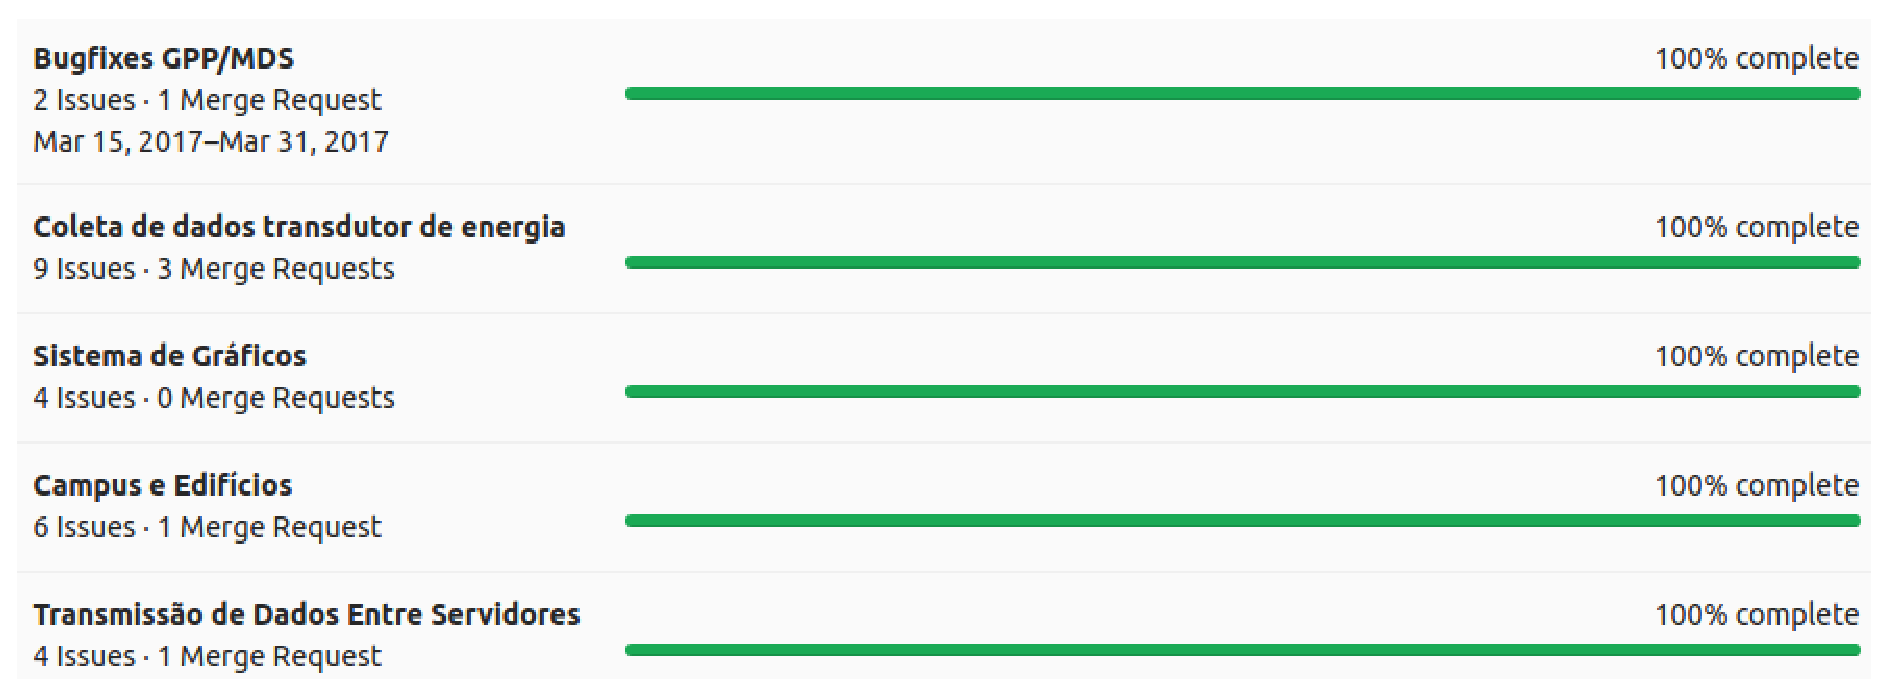
\includegraphics[keepaspectratio=true,scale=0.51]{figuras/milestones.eps}
    \caption{\textit{Milestones} realizadas durante as duas \textit{releases} do projeto.}
    \label{milestones}
\end{figure}

\section{Visão Geral do Desenvolvimento}
O desenvolvimento da parte inicial do projeto foi marcado por duas \textit{releases}, sendo estas:

\begin{itemize}
    \item \textit{Release} 1: 20/07/2016 a 25/11/2016;
    \item \textit{Release} 2: 06/03/2017 a 23/06/2017.
\end{itemize}

\subsection{\textit{Release} 1}
A primeira \textit{release} teve início com um estudo aprofundado sobre o equipamento de medição de energia que seria utilizado. Após o estudo, foi definida a arquitetura inicial do projeto e realizado um pequeno protótipo funcional, Figuras \ref{dados02} e \ref{dados01}, que conseguia efetivamente coletar os dados de energia.

\begin{figure}[!htb]
    \centering
    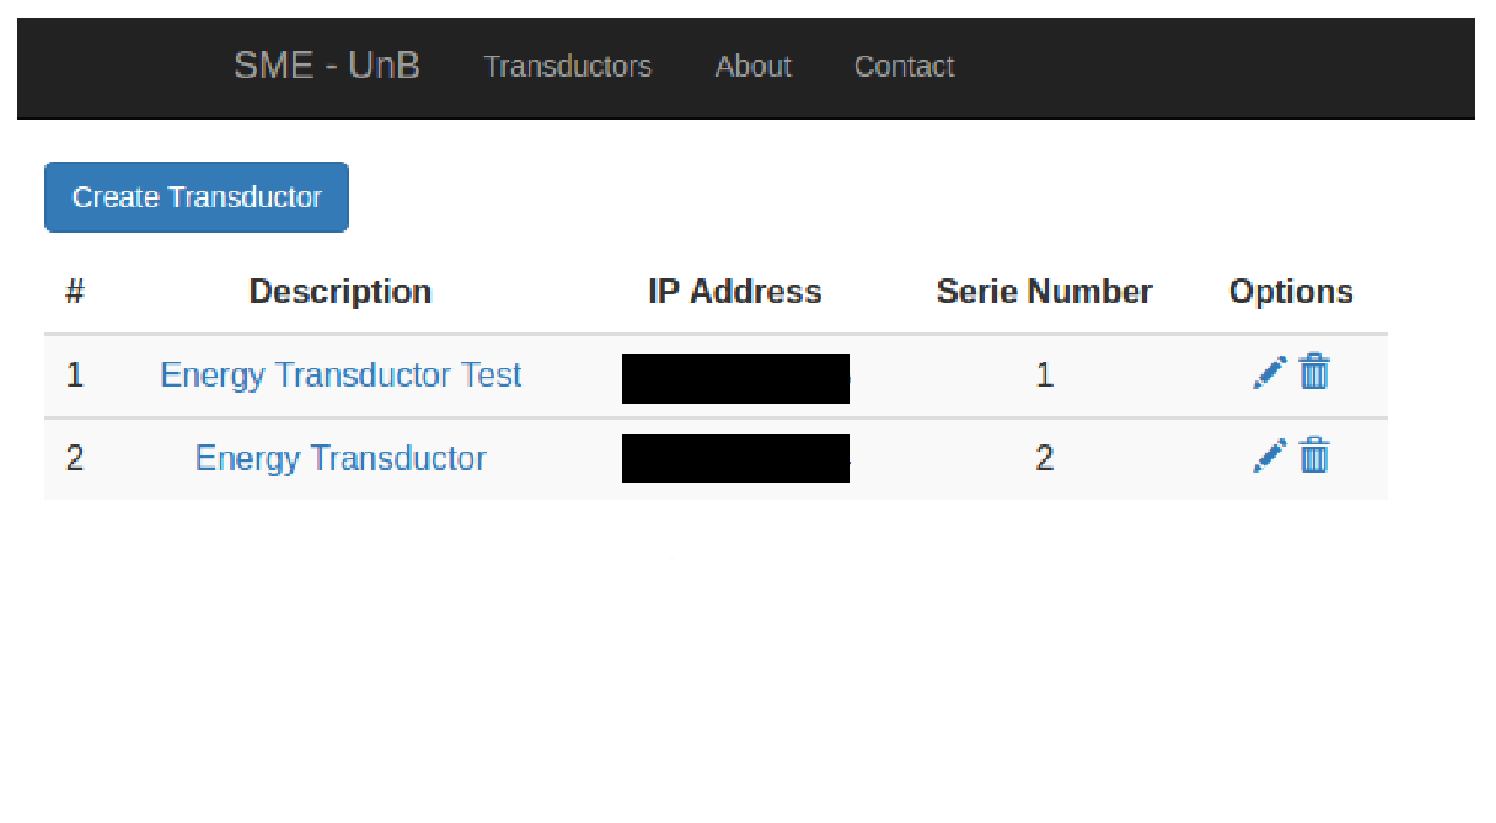
\includegraphics[keepaspectratio=true,scale=0.5]{figuras/coleta_dados_02.eps}
    \caption{Protótipo para apresentação dos transdutores \textit{release} 1.}
    \label{dados02}
\end{figure}

\begin{figure}[!htb]
    \centering
    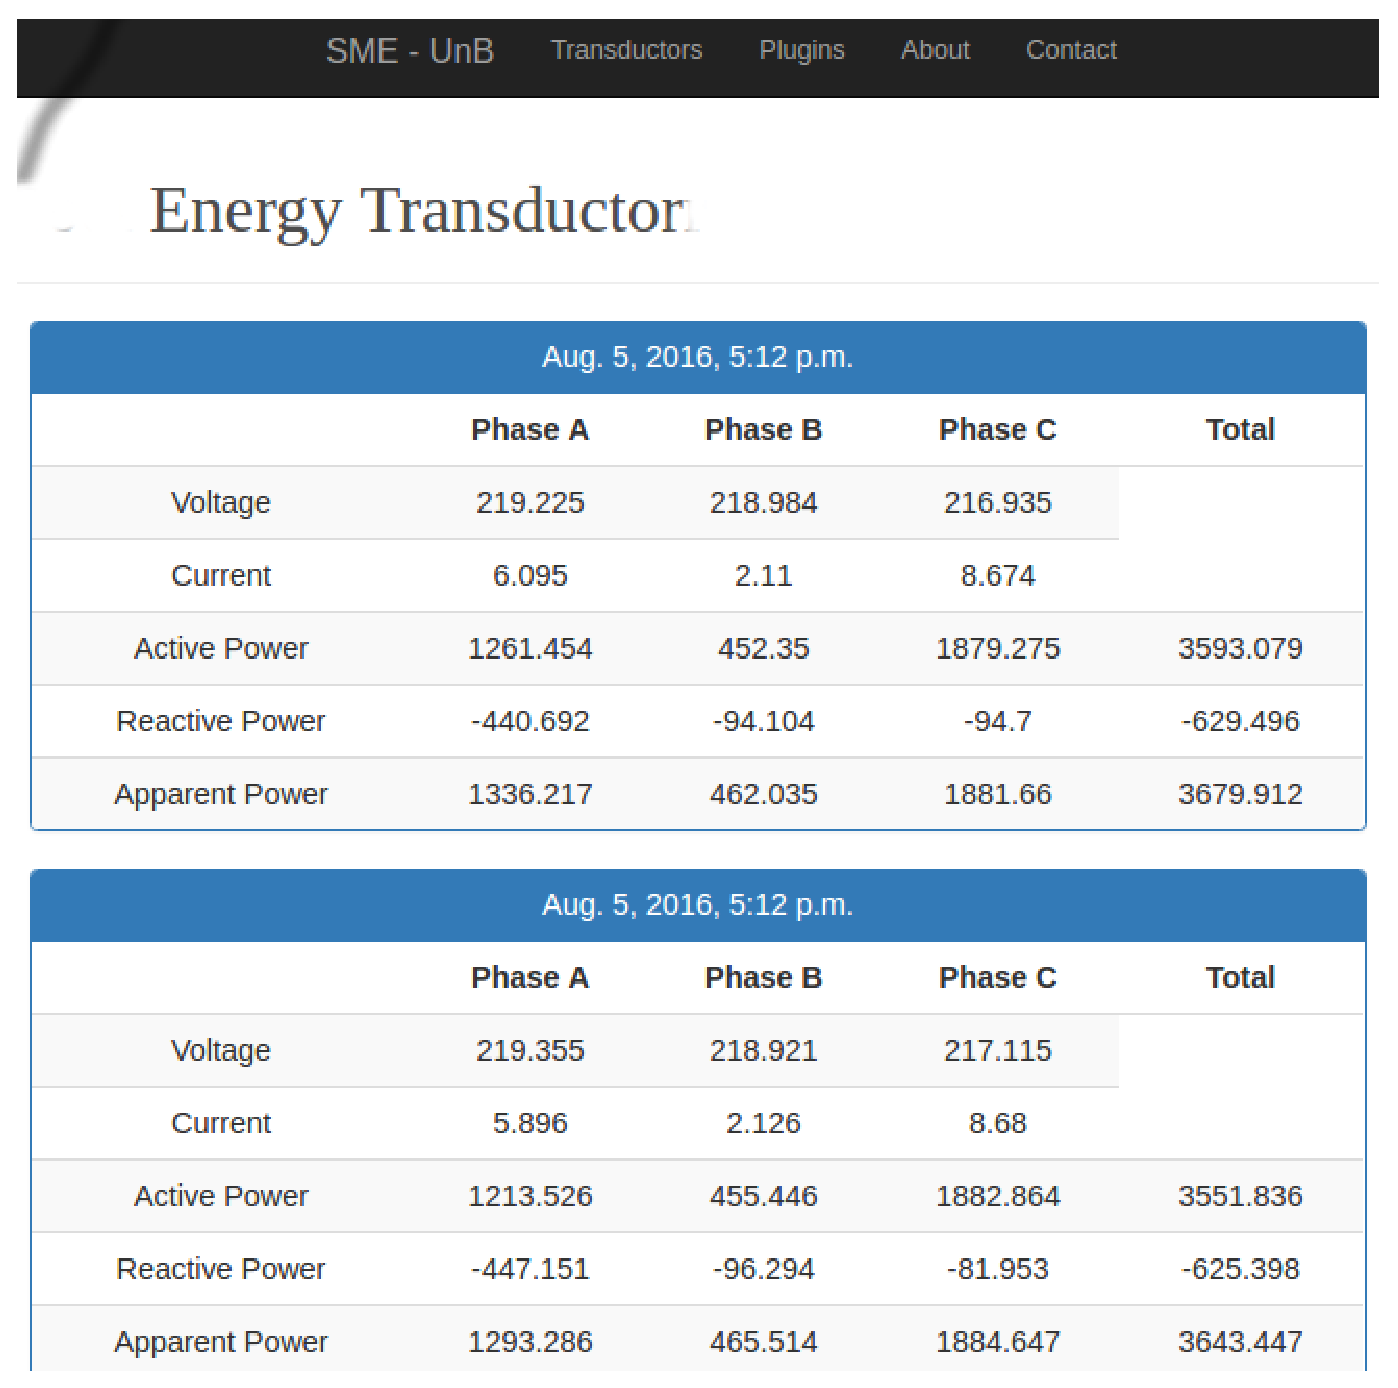
\includegraphics[keepaspectratio=true,scale=0.5]{figuras/coleta_dados_01.eps}
    \caption{Protótipo para apresentação medições de energia \textit{release} 1.}
    \label{dados01}
\end{figure}

Foi realizado um guia de instação para o ambiente de desenvolvimento no repositório, utilizando a ferramenta Vagrant\footnote{\url{https://www.vagrantup.com/}}. Esse guia objetivava tornar mais acessível o projeto a programadores que estivessem dispostos a realizar novas contribuições.

Uma vez que o código estava sendo escrito na linguagem Python 2.7, procurou-se sempre utilizar suas convenções para boas práticas de programação, definidas pela PEP 8\footnote{\url{https://www.python.org/dev/peps/pep-0008/}}. A ferramenta utilizada para realizar a verificação dessas normas foi o flake8\footnote{\url{https://pypi.python.org/pypi/flake8}}.

Diversos testes unitários foram realizados a cada término de uma funcionalidade, objetivando uma cobertura de no mínimo 90\%. Os testes foram escritos utilizando o módulo \textit{unittest} do próprio Python.

Pequenos erros eram encontrados nas funcionalidades, conforme seus testes unitários eram escritos. Após identificado os motivos desses erros, eles eram corrigidos.

Utilizou-se a biblioteca \textit{mock}, do \textit{unittest}, para que fosse possível definir determinados comportamentos em métodos que utilizassem um outro método durante sua execução, objetivando um maior desempenho na hora de executar a suíte de testes e unitariedade dos métodos.

Com o auxílio do serviço Gitlab CI, foi possível realizar de maneira fácil a integração contínua do projeto. Esse serviço utiliza como princípio um \textit{Runner}, que se baseia em uma máquina virtual isolada, responsável por realizar um \textit{Job}. Um \textit{Job} consiste na execução de comandos pré-definidos no arquivo padrão \textit{.gitlab-ci.yml}.

Diversas decisões arquiteturais foram realizadas no decorrer da \textit{release}, conforme as necessidades de implementação iam surgindo, objetivando cada vez mais modularizar e trazer maior robustez ao sistema.

Com o auxílio da ferramenta \textit{cron}, foi possível realizar a coleta de dados de forma temporizada.

Um ponto importante a se destacar, referente à primeira \textit{release}, foi o da colaboração provinda por alunos de duas disciplinas aplicadas pelo curso de Engenharia de Software no campus UnB-Gama: Gestão de Projetos e Portfólio de Software e Métodos de Desenvolvimento de Software. As disciplinas em questão eram includentes e realizadas em conjunto. Os incrementos de software providenciados ao projeto foram, em sua grande parte, referentes à gerência de usuários e autenticação.

A cobertura total de código obtida ao fim da \textit{release} 1 foi de 95\%.

\subsection{\textit{Release} 2}
A segunda \textit{release} teve início com uma forte refatoração sobre os incrementos de software provindos das equipes de GPP e MDS. Em conjunto, visto que o projeto estava em Python 2.7, realizou-se uma mudança para Python 3.5.

Com o projeto em Python 3.5, a autenticação do sistema foi modificada para ser realizada por e-mail, ao invés de nome de usuário.

Realizou-se um novo \textit{layout} para o sistema, visto que o anterior não estava esteticamente agradável.

Um gráfico de linhas foi realizado, utilizando a biblioteca Matplotlib\footnote{\url{https://matplotlib.org/}}, para que fosse possível visualizar as medições de um período específico de maneira mais fácil.

A gerência de usuários foi aprimorada, com a adição de algumas permissões, para que fosse possível ter diferentes níveis de acesso na aplicação.

Realizou-se um protótipo de API para realizar a comunição inter-campi e adicionado o conceito de conteinerização ao projeto, por meio do Docker.

A cobertura total de código obtida ao fim da \textit{release} 2 foi de 93\%.

\section{Implantação}
Não foi possível colocar o SMI-UnB em produção, visto que muitas funcionalidades importantes ainda precisam ser desenvolvidas, porém, algumas de suas funções importantes foram implementadas com sucesso.

Utilizou-se alguns dos conhecimento provindos do \textit{Devops} para auxiliar na distribuição do SMI-UnB. O \textit{Devops} é um processo de desenvolvimento de software que valoriza comunicação e colaboração entre gerentes de produto, desenvolvedores de software e outros profissionais. O \textit{DevOps} também automatiza os processos de integração de software, testes, implantação e mudanças de infraestrutura \cite{loukides_2012}.

Utilizou-se o Docker \cite{docker} para que fosse possível criar um ambiente unificado para o sistema, visando evitar futuros problemas de implantação.

O Docker é uma plataforma de contêiners de software. Um contêiner, Figura \ref{container}, possui empacotado tudo que é necessário para se executar um software completo ou parte dele. Diferente das máquinas virtuais, os contêiners são executados em uma mesma máquina, compartilhando o \textit{kernel} do seu sistema operacional, sendo que cada um terá seu processo isolado no espaço de usuário.

\begin{figure}[!h]
    \centering
    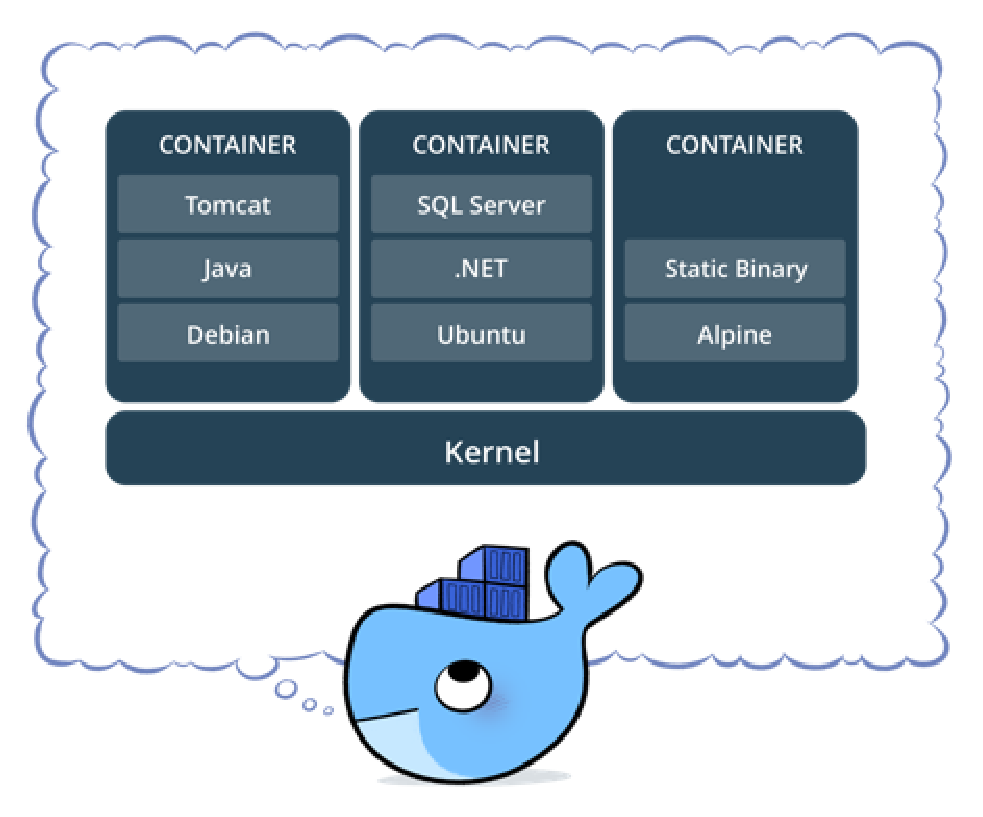
\includegraphics[keepaspectratio=true,scale=0.8]{figuras/container.eps}
    \caption{Exemplo de contêiners providos pelo Docker. Fonte: \cite{docker} }
    \label{container}
\end{figure}

Para Tanenbaum \cite{tanenbaum_2007}, o sistema operacional é a peça mais básica de software e opera em modo núcleo, possuindo acesso completo a todo o \textit{hardware} e ao conjunto de instruções oferecidos pela máquina. O resto do software opera em modo usuário, onde é disponível apenas um conjunto de instruções da máquina para execução.

Realizou-se um ambiente para testes no campus UnB-Gama, que possuía o SMI-UnB instalado como um serviço, objetivando averiguar o que havia sido implementado.